\documentclass[../main.tex]{subfiles}
\title{Network Models}

\AtBeginSection[] % Do nothing for \section* %
{
\begin{frame}<beamer> 
  \frametitle{Agenda}
  \tableofcontents[currentsection] 
\end{frame}
}


\begin{document}
% ==============================
\begin{frame}
  \maketitle
\end{frame}


\begin{frame}{Agenda}
  \tableofcontents
\end{frame}
% ==============================


\section{Introduction}
\label{sec:intro}

\begin{frame}{Introduction to the Model}
  \begin{itemize} \parskip3mm \justifying
    \item<only@1> The origin of transportation models dates back to 1941 when F.L. Hitchcock presented a study entitled ``The Distribution of a Product from Several Sources to Numerous Localities.'' The presentation is regarded as the first important contribution to the solution of transportation
    problems. 
    \item<only@1> In 1947, T.C. Koopmans presented a study called ``Optimum Utilization of the Transportation System''. 
    \item<only@1> These two contributions are mainly responsible for the development of  transportation models which involve a number of shipping sources and a number of destinations.
    \item<only@2> Each shipping source has a certain capacity and each destination has a certain requirement  associated with a certain cost of shipping from the sources to the destinations. 
    \item<only@2>  The objective is to minimize the cost of transportation while meeting the requirements at the destinations. Transportation problems may also involve movement of a \alert{product from plants to warehouses, warehouses to wholesalers, wholsalers to retailers and retailers to customers.} 
    \end{itemize}
\end{frame}

\begin{frame}{Assumptions In The Transportation Model}
  \begin{enumerate} \parskip3mm \justifying
    \item Total quantity of the ítem available at different sources is equal to the total requirement at different destinations. \item Item can be transported conveniently from all sources to destinations.
\item The unit transportation cost of the item from all sources to destinations is certainly and pecisely known.
\item The transportation cost on a given route is directly proportional to the number of units shipped on that route.
\item The objective is \alert{to minimize the total transportation cost} for the organisation as a whole and not for individual supply and distribution centres.
  \end{enumerate}
\end{frame}

\begin{frame}{Definition}
  Suppose that there are $m$ sources and $n$ destinations. Let $a_i$ be the number of supply units available at source $i(i = 1, 2, 3, \ldots, m)$ and let $b_j$ be the number of demand units required at destination $j(j = 1, 2, 3, \ldots, n)$. Let $c_{ij}$ represent the unit transportation cost for transportating the units from source $i$ to destination $j$.

  The objective is to determine the number of units to be transported from source $i$ to destination $j$ so that the total transportation cost is minimum. In addition, the supply limits at the sources and the demand requirements at the destinations must be satisfied exactly.
\end{frame}

\begin{frame}{Definition}
  If $x_{ij}(x_{ij} \geq 0)$ is the number of units shipped from source $i$ to destination $j$, then the equivalent linear programming model will be Find $x_{ij}(i = 1, 2, 3, \ldots, m; \,\, j = 1, 2, 3, \ldots , n)$ in order to

  \[ \min Z = \sum_{i=1}^{m} \sum_{j=1}^{n} c_{ij}x_{ij}\]
  \begin{flalign*}
    \text{subject to} \quad & \sum_{j=1}^{n} x_{ij} = a_i,  \quad i=1,2,3,\ldots,m,\\
    \text{and} \quad& \sum_{i=1}^{m} x_{ij} = b_j,  \quad i=1,2,3,\ldots,n,\\
    \text{where} \quad& x_{ij} \geq 0 
  \end{flalign*}

\end{frame}


\begin{frame}{Matrix Terminology}
  
  {\centering
  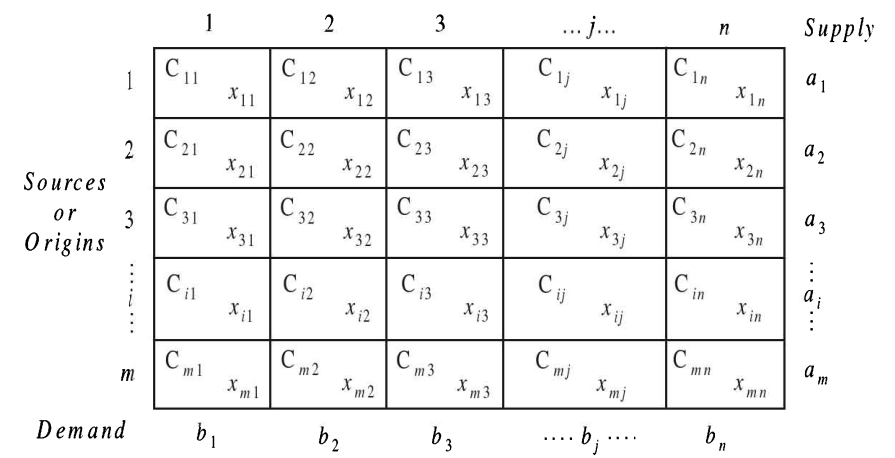
\includegraphics[scale=0.4]{matrix-transportation.png}
  \par}
\end{frame}

\begin{frame}{Matrix Terminology}

     The matrix used in the transportation models consists of squares called ``cells'', which when stacked form ``columns'' vertically and ``rows'' horizontally. The cell located at the intersection of a row and a column is designated by its row and column headings. Thus the cell located at the intersection of row A and column 3 is called cell (A, 3). Unit costs are placed in each cell

  {\centering 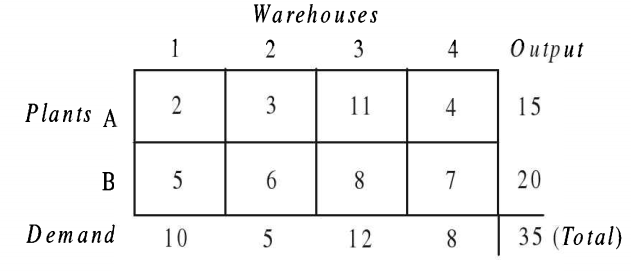
\includegraphics[scale=0.5]{cells.png}\par}
\end{frame}

\begin{frameExample}{Transportation Problem}{}
  % EXAMPLE 3.5-1 {Transportation Problem}
    \only<1>{
  A dairy firm has three plants located throughout a state. Daily milk production at each plant is as follows:

  \begin{itemize}
  \item[] Plant 1 \textellipsis 6 million litres,
  \item[] plant 2 \textellipsis 1 million litres, and
  \item[] plant 3 \textellipsis 10 million litres.
  \end{itemize}

Each day the firm must fulfil the needs of its four distribution centres. Milk requirement at each centre is as follows:
\begin{itemize}
\item[] Distribution centre 1 \textellipsis 7 million litres,
\item[] distribution centre 2 \textellipsis 5 million litres,
\item[] distributoin centre 3 \textellipsis 3 million litres, and
\item[] distribution centre 4 \textellipsis 2 million litres.
\end{itemize}
 }

 \only<2>{
   Cost of shipping one million litres of milkfrom each plant to each distribution centre is given in the following table in hundreds of dollars:
  
   {\centering 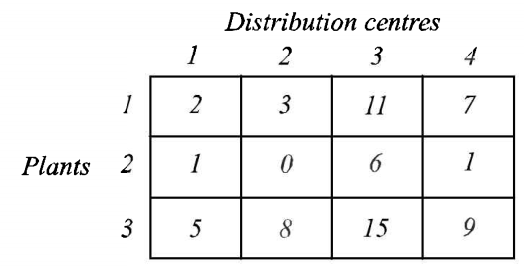
\includegraphics[scale=0.5]{example-3-5-1.png}\par}
 }

 \only<3>{
   \begin{enumerate}[(i)] \parskip3mm \justifying
   \item  Show that the problem represents a network situation.
   \item  Formulate the mathematical model for the problem.
   \item  The dairy firm wishes to determine as to how much should be the shipment from which milk plant to which distribution centre so that the total cost of shipment is the minimum. Determine the optimal transportation policy.
   \end{enumerate}

 }
  
\end{frameExample}




\end{document}
